%%% DO NOT CHANGE ANYTHING FROM HERE %%%
\documentclass[11pt]{article}
\makeatletter

\usepackage{comment} % enables the use of multi-line comments (\ifx \fi) 
\usepackage{lipsum} %This package just generates Lorem Ipsum filler text. 
\usepackage{graphicx}
\usepackage{fullpage} % changes the margin
\usepackage{setspace}
\doublespace

\begin{document}
%%% TO HERE; MAKE CHANGES BELOW. %%%

\noindent
\normalsize Lucas Estrada, Charlie Ide \\
\normalsize   Due Date: December 13, 2019 \\\\
\noindent
\centerline{\Large\textbf{Project: SQL Injection}}

\section*{Abstract}
Our attack is a SQL injection against a website that we produced. Unprotected SQL databases are vulnerable to craftily written inputs that allow hackers to inject their own code to the SQL Query. This affects all resources because the hacker can inject any code and write any query that they so choose. Any attacker looking to gain confidential information or alter a protected database could gain from this attack. The attack is quite simple to perform against an unprotected database for anyone who understands SQL syntax. 

\par The consequences are quite severe because an attacker could delete a whole database or gain access to confidential information like bank account info. The attack was invented in 1998 and is now one of the most common vulnerability in the internet. The attack works by writing malicious queries to a database end point on a website such as a login database. It is relatively easy to counteract this by sanitizing inputs or even better, using prepared statements. Although simple this is a very significant attack because of the prevalence of SQL databases for many online applications that require databases. 

\section*{What is the vulnerability?}
We are studying SQL injection attacks, a form of attack in which users (potentially malicious) are given the chance to enter input into fields that are used to query SQL databases. If the user has a proper understanding of the syntax of SQL and the commands that are being used to issue queries then they can write their input parameters as to hijack the query and make the database perform a different action than is intended by the database owner.

\section*{What resources are affected?}
This vulnerability affects SQL databases that allow users to input data into query fields. This tends to take the form of online databases with search functionality that are powered by a SQL server. Login databases are most common.

\section*{In what way are resources affected? (confidentiality, integrity/authorization, availability, non-repudiation)}
Confidentiality can be affected if certain records of the database are intended to remain private and a user structures a query as to obtain access to these records. Integrity is affected because a user could structure a query to edit data in the database. Availability is affected because a user could drop tables and destroy the data stored, thus making it unavailable to users. Non-repudiation seems to be unaffected since all SQL queries are traceable to their author.

\section*{Who would gain from undertaking such an attack? What kind of background or resources does that person need?}
An attacker could gain access to confidential information stored on a SQL server that could be lucrative. This could take the form of private personal information such as bank pins or proprietary data powering a machine learning tool. It could also be used to sabotage organizations by destroying their data or corrupting it. A person conducting this attack would just need a regular computer and understanding of how SQL queries work and their syntax. They would then need to find a vulnerable database.

\section*{Is the attack difficult?}
If one finds a vulnerable database that does not sanitize inputs and returns all results of a query to the user or perform any other actions a user might enter into the query, then the attack is relatively simple to perform. Dropping a whole database can be done with just a line of code entered in a specific format into the database.

\section*{Are the consequences of the attack mild or severe?}
The consequences of the attack can be quite severe from the complete destruction of a database to hackers gaining complete access to the data stored. 

\section*{What is the history of this attack? Who invented it (if we know)? Is it hypothetical or “in the wild”? Has it ever been deployed maliciously?}
In 1998, Jeff Forristal published an article in Phrack Magazine describing the proposed attack. It is still one of the most common attacks against web applications because of its ease and how common SQL servers are used to power databases on web applications. There are numerous examples of where this attack has been deployed maliciously. One early example came in 2002 when an activist discovered a hacker could steal over 200,000 credit card numbers from Guess.com using a SQL injection attack. \newline
Sources \newline http://phrack.org/issues/54/8.html\#article \newline
https://www.securityfocus.com/news/346


\section*{How does it work?}
SQL Injection is a method of web attack where users can insert executable SQL commands into existing databases. This potentially allows attackers to gain access to privileged server data as well as the authority to delete the entire database. The way this attack works is based on the assumption that a database or website utilizing SQL asks for input, say a username or password, and then uses that input without sanitizing it. The user can then input valid SQL code if they have a good understanding of how a query command is written for this particular site's source code. The diagram below (Figure 1) shows two examples of this type of attack, showing how if the underlying architecture of the database does not check user input for malicious code, they can gain access to the system or mess with the code.\\

\begin{figure}[t]
\center{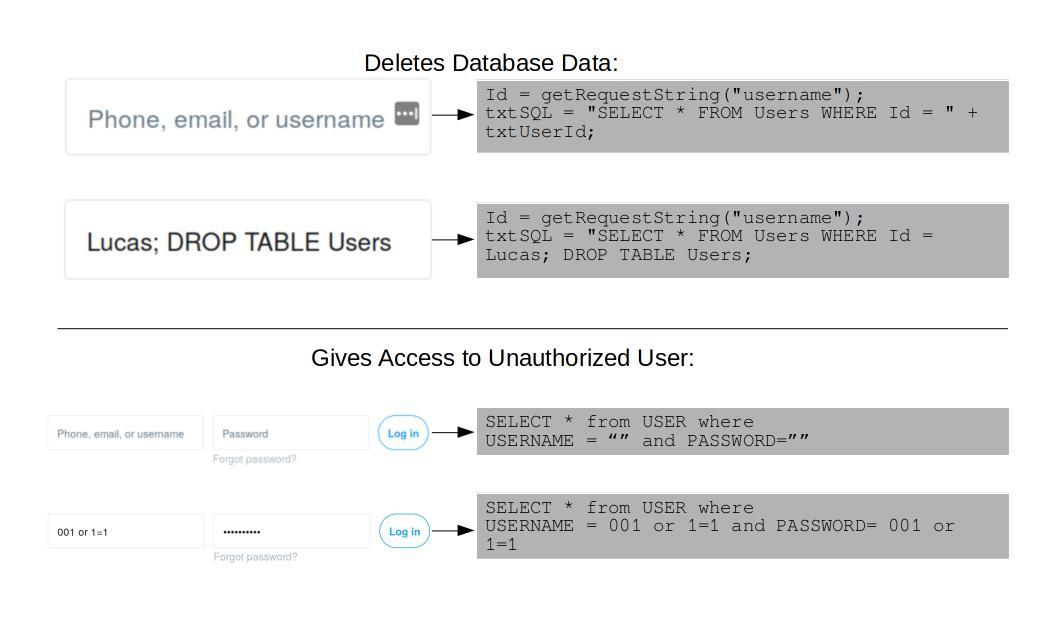
\includegraphics[width=\textwidth]{diagram.jpg}}
\caption{\label{fig:my-label} Example of an SQL Injection attack, using two different methods. Example 1 (Upper) uses batching of SQL code, while Example 2 (Lower) uses modification of existing logical operating statements.}
\end{figure}
\\

In the first example, the attacker takes advantage of SQL batching, where multiple lines of code can be executed with semicolon separation. This allows the attacker to delete the entire table of users in this case because the user input is taken directly into the code and run as if it were a continuation of the line. In the second example, the attacker gains privileged access by circumventing the username and password checking against the database. By inserting "or 1=1" after a username and password, an attacker can ensure that the login attempt is successful without having an accepted password, as 1=1 will always be true.\\

However, with both of these examples it is important for the attacker to have access to the source code to identify the injection technique that will work. If the input in the first example was used in the second example, and vice versa, the attack would fail. Similarly, if a site does not use SQL an SQL injection would fail. Thus, an attacker must either have access to the source code or be persistent in trying such an attack on different sites that could potentially be vulnerable to this type of attack. In the case that an attacker does not have the source code they can often make progress in crafting a SQL query using error messages as clues. When SQL queries are improperly formatted they will return error messages that will often be delivered to the hacker. These error messages can offer clues as to the underlying structure of the SQL query implementation that the hacker can then use to revise their inputs.\\

When crafting input it is important to first understand the structure of a SQL query. Many SQL database queries from inputs are structured something like 
$SELECT$ $*$ $FROM$ $database$ $WHERE$ $parameter$ $=$ $'INPUT';$, where input is the query entered by the user from their database end point. The $SELECT$ $*$ $FROM$ $database$ part of this statement selects all entries from a database that we specify. The $WHERE$ $parameter$ statement allows us to only choose those statements where a column value for that entry matches an input that we provide. In the case of cuteanimals.edu we match the animal name to an animal name input by the user. We should also notice that input is enclosed within quotation marks and that each SQL statement is terminated with a semicolon. We also know that SQL comments are marked with the $--$ symbol.  \\

Knowing this, we can terminate our input using a $';$ symbol and then write further lines of code or add statements to our SQL query. To gain full access to our cuteanimals.edu database we terminated our input value with a $'$ symbol but we then added the statement $OR$ $1=1;--$ This $OR$ statement is always true which means that we select all entries from our database, thus giving us access to the entire database rather than just one entry as the website was intended to give the user. The comment symbol eliminates any symbols such as stray $'$ or $;$ that are left in our SQL query. This is important to prevent syntax errors. While this might not be an issue for a database of cute animals, it would be an issue if we were storing sensitive information and a user was able to access others' information.\\

Another attack that we could have carried out would be to destroy the entire database using a $DROP$ $TABLE$ line. We could insert the input $';$ $DROP$ $TABLE$ $database;--$. This code would first close off our empty input and terminate that SQL statement. We then write a new SQL statement that drops our database, thereby destroying all the information that we had in our database. This attack would destroy the availability of our data. More generally this technique of terminating the intended query then writing new statements could be used to write any SQL code one wanted to the database. One could alter data, insert new entries, or do anything that a database administrator could otherwise do with this ability to directly write SQL code. \\

The simplicity of this type of attack makes it an attractive option for an actor trying to gain access to privileged data. No special resources are required as this is not a particularly time or space intensive attack. The resources computing resources needed are no greater than is required for standard use of web applications. Since all sites may not be vulnerable to this type of attack the main complexity comes from finding susceptible targets. This can be achieved by an exhaustive linear search of sites that an attacker may suspect uses SQL as the underlying login or database architecture. This is a similar attack as that undertaken by the hacker in the Cuckoo's Egg in which the hacker launches simple attacks against a wide variety of targets and just hopes that one of the system administrators failed to properly secure their systems. \\ 

Clearly this problem can be quite severe when a large database of valuable information is compromised. However, as we will learn in the next section SQL injections are not automatically protected by SQL servers but are quite easy to prevent if the system administrator is aware aware that they need to protect against these attacks. Because of this smaller databases implemented by more amateur web designers are more likely to be vulnerable, but large databases implemented by professionals storing valuable data are almost surely protected. Because of this attacking any high value targets would almost surely fail because anyone with an understanding of security would secure their database from this threat. \\

We do not have data on what proportion of web applications protect themselves from SQL injections using best practices however it is likely that hackers would need to try many websites to find a potential vulnerable database. Should they find such a database it is likely a lower value target built by less experienced developers. The most valuable resource hackers could harvest in this situation is users' passwords and emails. If our administrators didn't know to prevent SQL injections maybe they don't know to encrypt passwords either. Because of password reuse hackers could then try these login credentials on more valuable applications such as banking websites and Amazon to gain access to user accounts. \\ 

To implement this particular attack we built a website utilizing SQL databases and taking user input in an insecure manner. To accomplish this we will create a relatively simple site that allows users to look up cute animal pictures using the animal name. If the animal name is in our database then a picture of that animal will pop up to the screen. In this project we will be demonstrating a batch SQL vulnerability where the attacker inputs code similar to example 1 in the diagram, allowing them to delete our entire database of cute animal pictures from our server -- decimating the marketability and commercial value of "cuteaminals.edu". We expect the actual attack to be relatively easy, but creating the vulnerable website may be difficult depending on how we host it. Github, for example, only allows static websites to be hosted on their servers, preventing user input from affecting the site. This means that we cannot have users query our website as is necessary for a SQL attack. At this point we think that creating the example website locally on our devices and showing how the attack would work if the vulnerable page were hosted online should suffice for the scope of this project. 

\section*{Countermeasures}
To defend against this type of attack developers should always sanitize user input. This can be done in a variety of ways, but perhaps the easiest is to use SQL parameters when taking user input. This is known as using prepared statements. Prepared statements take input given at execution time and ensure that the input is taken literally and not as executable code. Other methods sanitizing input include checking for special characters that could be used for such an attack before accepting any user input. Additionally keeping one’s source code confidential prevents attackers from identifying inherent vulnerabilities in one’s code, but this is not a method to use instead of sanitizing input — always sanitize to prevent SQL Injection!

\section*{Conclusion}
SQL attacks are both one of the simplest attacks to carry out and one of the most common vulnerabilities on web applications. This means that it is very easy for random unsophisticated hackers exploring the internet to stumble upon naive databases and exploit them. Luckily, they are also one of the simplest to defend against using prepared statements so long as the application designer is aware of the vulnerability and countermeasures. \\

When creating our injection we discovered (luckily for us because it made our attack possible) that inputs are not automatically sanitized and that coders need to manually add prepared statements to prevent SQL injection. It seems like the implementation of PHP or mySQL could be altered so that it automatically prepares SQL inputs. If this alteration were made then this would easily prevent the majority of common SQL injection attacks. If this change in underlying implementation were not possible then the next best solution would be to widely educate web designers so that they understand they need to sanitize their inputs. In that regard nobody had done more for SQL database safety than Randall Munroe with his Bobby Tables cartoon which has widely publicized the danger of SQL injection and need to santize inputs. 

\section*{Sources}
https://xkcd.com/327/ \\
https://www.owasp.org/index.php/SQL\_Injection \\
https://www.w3schools.com/sql/sql\_injection.asp \\
https://www.geeksforgeeks.org/sql-injection-2/

\end{document}